\section{Co je to multiplatformní vývoj?}
Multiplatformní vývoj je nadále žhavým tématem v diskuzích uvnitř komunit vývojářů desktopových i mobilních aplikací. Jedná se o přístup, který umožňuje vývojářům napsat program jednou, ale být jej schopen spouštět na více platformách. Pro splnění definice však již není podstatné, na kolika platformách může program běžet, pakliže je jich více než jedna. Tedy i aplikace, která dokáže běžet pouze na dvou platformách, je z hlediska této definice multiplatformní.

Na tomto místě by šlo namítnout, že i aplikace, která je napsána pro každou platformu zvlášť, je multiplatformní, neboť jí lze spouštět na více systémech. Je to do jisté míry pravda, nicméně pokud se na to podíváme z jiného úhlu, můžeme takový přístup označit za vývoj aplikací, které se podobají, ale nejedná se o programy totožné.

Multiplatformní přístup je tedy způsob, jak využít jeden zdrojový kód, který jsme schopni provozovat (s minimálními úpravami) na různých platformách a operačních systémech. Pro tento přístup se v angličtině vžilo heslo „write once, run everywhere“. 

Jedním z často používaných dělících kritérií, pomocí kterých můžeme multiplatformní software rozlišovat, je kritérium způsobu jejich kompilace a následného běhu na samotné platformě.

\begin{enumerate}
	\item Zdrojový kód je nutno zkompilovat pro každou platformu zvlášť. Poté je tedy nutno udržovat repozitář s různými instalačními balíčky pro jednotlivé platformy.
	\item Zkompilování zdrojového kódu pouze jedinkrát a jeho následný běh na uživatelově platformě pomocí nějakého interpreteru či run-time prostředí, které je součástí systému.
\end{enumerate}

Příkladem multiplatformních aplikacích je  vývojářské prostředí Eclipse, internetový prohlížeč Opera, Google Earth apod.

Jak již bylo řečeno, způsobů jak multiplatformně vyvíjet je mnoho. Pro tvorbu multiplatformní desktopové aplikace je možno využít standardního programovacího jazyka (pro který existuje kompilátor na více platformách) spolu s frameworkem, který umožňuje multiplatformní vývoj (nejen) GUI. Mezi takové UI toolkity můžeme zařadit například Qt, wxWidgets nebo GTK+. 

Kapitola sama pro sebe je Java. Java je platformou umožňující vývoj aplikací zcela nezávislých na operačním systému. Tato technologie je skutečným zosobněním přístupu „write once, run everywhere“. Nutno však v zápětí dodat, že „everywhere“ je omezeno přítomností Java Virtual Machine. Programy napsané v Javě totiž nejsou závislé na konkrétním operačním systému, ale právě na speciálním prostředí (JVM), které zdrojový kód (Java bytekód) interpretuje.

Ačkoliv je Java velmi oblíbenou vývojářskou platformou, nestala se nikdy všudypřítomnou technologií, která překoná rozdíly mezi platformami, jak se mnozí domnívali. O důvodech můžeme spekulovat. Jedním z nich je zcela nepochybně nenativní chování javovských aplikací. Programy v Javě totiž na dané platformě málokdy působí jako nativní aplikace, což představuje značnou překážku k jejich širokému přijetí. I přes snahy o řešení (například pomocí knihovny Java Swing) se tento problém stále nepodařilo zcela překonat.

Nezřídkakdy se můžete setkat s názorem, že „HTML5 je nová Java“ \cite{why_html5_java}. Toto tvrzení vychází zejména z faktu, že HTML5, stejně jako Java, splňuje paradigma „write once, run everywhere“. Na rozdíl od Javy je však vývoj v HTML5 podstatně jednodušší a výkon aplikací se neustále zlepšuje (zejména díky výkonnějším JavaScriptovým enginům v internetových prohlížečích). Další předností HTML5 aplikací je jejich snadná dostupnost pro koncového uživatele. Nemusí instalovat víc než webový prohlížeč a znát tu správnou URL. 

Zásadním argumentem, proč je HTML5 novou Javou, je však podle mě něco jiného. Je to zejména dramatický nástup mobilních zařízení. „Write once, run everywhere“ pro javovské aplikace v mobilním světě neplatí. Z předních hráčů na trhu se Java Virtual Machine vyskytuje pouze na Androidu, na ostatních platformách si tudíž javovské aplikace nespustíte. Naopak HTML5 je díky všudypřítomnosti webového prohlížeče skutečně multiplatformní technologií i z pohledu mobilního světa. 

Samozřejmě by někdo mohl namítnout, že porovnávání Javy a HTML5 poněkud kulhá, neboť funkcionalita, kterou dává vývojářům k dispozici Java, je oproti HTML5 obrovská. Avšak HTML5 obsahuje (a nadále přidává) zejména ty funkce, které najdou uplatnění i v chytrých mobilních telefonech. A z těch již zase tak mnoho nechybí. HTML5 přebírá pozici Javy právě proto, že je úspěšné i na poli mobilních telefonů.

\section{Argumenty pro multiplatformní přístup}
V této části bych se rád podrobněji zaměřil na důvody, které vedou vývojáře k zahrnutí multiplatformního řešení do svých úvah. Pokusím se zde nastínit argumenty, které se v této souvislosti nejčastěji skloňují.

\subsection{Možnost cílit na široké spektrum platforem najednou}
Tento důvod byl podle výzkumu společnosti VisionMobile uváděn vývojáři nejčastěji \cite{visionmobile_survey}. 60 \% z nich konstatovalo, že právě širší záběr, který jim multiplatformní přístup přináší, je přesvědčil k využití některého z multiplaformních nástrojů.

Velké společnosti stojící za platformami jako je Android či iOS se velmi snaží, aby vývojáři vyvíjeli exkluzivně pro jejich platformu. Přítomnost těch nejžádanějších aplikací výhradně pro jednu platformu jí totiž přináší značnou konkureční výhodu na trhu. V zájmu těchto hráčů proto není, aby bylo možné aplikace snadno vyvíjet na více platforem najednou. Naopak méně rozšířené systémy jako je Windows Phone, Samsung Bada, RIM a další mají eminentní zájem na tom, aby bylo pro jejich systém dostupné co největší množství aplikací bez zbytečného čekání. Takzvaný „time-to-market“ je totiž u těchto platforem často mnohem větší než u velkých hráčů,[c] protože nativní vývojáři se logicky snaží prvně zasáhnout co největší část trhu, která je okupována právě iOS a Androidem. 

Možnost rychle zasáhnout tzv. „long tail“ je tedy pro vývojáře velice lákavá. Mohou bez zbytečných prodlev rychle oslovit prakticky celý trh a nemusí tak dávkovat marketingovou podporu podle toho, na které platformě jejich aplikace právě běží. O jejich aplikaci mohou mluvit všichni.

\subsection{Nižší náročnost na zdroje}
Náročnost na zdroje je klíčový faktor zejména pro společnosti, které aplikace vyvíjejí. Pokud chtějí být s aplikací opravdu úspěšní, musí s ní oslovit co nejširší spektrum uživatelů. To v dnešní době znamená mít verzi pro iOS, Android a Windows Phone. Dělat nativní aplikaci pro každý z těchto systémů znamená platit tři týmy vývojářů, protože pro každou platformu se programuje jiným programovacím jazykem, systém má jiná API volání a podobně. Zároveň je velmi neobvyklé, aby jeden vývojář ovládal na solidní úrovni technologie pro všechny tři platformy.

Ale problém není jen v kódování. Vyvíjet pro tři různé platformy znamená udržovat tři různé sady zdrojových kódů, trackování bugů pro každou z nich zvlášť a podobně. Zároveň účinná synchronizace mezi týmy klade další požadavky na lidské zdroje. Zajistit, aby všechny tři verze měly stejné vlastnosti, dodržovaly stejná designová paradigmata a zároveň se neodchylovaly od časového harmonogramu, je poměrně obtížný úkol.
\\ \\
\textit{\uv{Zjistili jsme, že použitím multiplatformního nástroje jsme schopni v průměru zredukovat náš ‚time to market‘ o 70\%,}} tvrdí Paulius Uza, výkonný ředitel společnosti InRuntime \cite{visionmobile_survey}.
\footnote{“We have found that by using cross-platform tools our time to market is reduced by 70\% on average,” remarks Paulius Uza, CEO of development house InRuntime \cite{visionmobile_survey}.}	

\subsection{Nižší finanční náročnost}
S předchozím bodem přímo souvisí i nižší finanční náročnost. Je zřejmé, že když budete zaměstnávat méně vývojářů, kteří pro vás aplikaci vyvíjejí, i vaše náklady budou nižší. Není to však jen o samotném vývoji. Po vypuštění hotové aplikace na trh je nutno zajistit podporu pro její uživatele. Z hlediska rozpočtu je značný rozdíl, zda-li musíte obhospodařovat jednu sadu se zdrojovými kódy nebo tři.

Podle společnosti VisionMobile stojí vývoj pro každou další platformu v průměru 50 \% původních nákladů \cite{visionmobile_survey}. Nejedná se tedy rozhodně o malé částky a každou rozpočtově odpovědnou firmu tento fakt nutí k zamyšlení, jak vyvíjet pro více platforem levněji.

\subsection{Menší vstupní bariéry}
K tomuto argumentu si nejprve uveďme dvě poznámky. Zaprvé, jazyky, ve kterých se vyvíjí nativní aplikace jsou poměrně obtížné na naučení. Názorným příkladem je v tomto ohledu Objective-C, který se vyznačuje nejen poměrně neobvyklou syntaxí, ale zároveň obsahuje množství značně neobvyklých návrhových vzorů a doporučení, která jsou poměrně obtížná na pochopení. I to je důvodem, proč je na trhu v současnosti převis nabídky nad poptávkou po vývojářích mobilních aplikací.

Neméně důležitým faktorem je poměrně široká masa webových vývojářů, která se na trhu vyskytuje. Webové technologie jsou v současnosti velmi oblíbené a to především díky strmému nárůstu popularity celého Internetu v minulé dekádě. Vývoj pomocí webových technologií je poměrně jednoduchý, neboť se při něm vývojář pohybuje na vysoké úrovni abstrakce. Díky tomu je možno vyvíjet webové aplikace rychle a levně.

Tohoto faktu šikovně využívají tvůrci multiplatformních řešení. Snaží se zasáhnout právě široké obecenstvo v řadách webových vývojářů tím, že maximálně snižují vstupní bariéry, které by jim mohly bránit ve vývoji mobilních aplikací. Drtivá většina multiplatformních nástrojů proto využívá pro vývoj mobilních aplikací právě webové technologie HTML[e], CSS a JavaScript. Pro přístup k nativním funkcím telefonu nabízí tyto nástroje jednoduchá API[g]. Že se jim tento přístup vyplací, dokládá i výzkum společnosti VisionMobile, který zjistil, že více jak 60 \% vývojářů, kteří využívají některý z multiplatformních nástrojů, má více jak 5 let zkušeností s webovým vývojem. Stejně tak při pátrání po důvodech, které vedly vývojáře k využití některého z multiplatformních nástrojů, byla jako druhá nejčastější odpověď uváděna právě možnost využít již naučené technologie \cite{visionmobile_survey}.

\section{Slabiny multiplatformního přístupu}
Pokud zmiňujeme přednosti multiplatformního přístupu, neměli bychom zapomínat ani na slabiny, které stále brání jeho širšímu rozšíření.

\subsection{Slabší výkon}
Slabší výkon je nejčastěji uváděným důvodem pro zavržení multiplatformního nástroje \cite{visionmobile_survey}. Vzhledem k tomu, že drtivá většina multiplatformních nástrojů závisí na nějaké mezivrstvě (ať už je to jakýsi most u hybridních aplikací, nebo runtime), není slabší výkon takto vytvořených aplikací příliš překvapivý.

\subsection{Omezený přístup k nativním funkcím zařízení}
Pravdou je, že ze své podstaty budou multiplatformní nástroje vždy o několik kroků pozadu oproti nástrojům pro nativní vývoj. Souvisí to právě s tím, že se multiplatformní nástroje snaží podporovat co nejvíce různých platforem. Z toho důvodu se musí omezovat na průnik množin funkcí, které tyto platformy nabízejí. Velice dobře tento problém popsal Steve Jobs ve svém otevřeném dopise společnosti Adobe „Thoughts on Flash“.
\\ \\
\textit{\uv{Z naší strastiplné zkušenosti víme, že položením vrstvy třetí strany mezi vývojáře a platformu, nevyhnutelně získáme aplikace podprůměrné kvality a vytvoříme tím překážky pro další rozvoj platformy. Pokud se vývojáři naučí být závislí na knihovnách a nástrojích třetí strany, mohou využívat nových vylepšení platformy až ve chvíli, kdy se třetí strana rozhodne je implementovat. Nemůžeme být vydáni na milost třetí straně, až se rozhodne umožnit našim vývojářům používat vylepšení, které v platformě uděláme. \\ \\
Problém se jenom zhorší, pokud třetí strana v rámci svého nástroje podporuje více platforem. Třetí strana pak nemusí implementovat nová vylepšení z jedné platformy až do chvíle, dokud jej neimplementují všechny platformy jež podporuje. Vývojáři aplikací pak mají přístup pouze k nejnižšímu společnému jmenovateli všech funkcí.}} Steve Jobs \cite{thoughts_on_flash}

\footnote{"We know from painful experience that letting a third party layer of software come between the platform and the developer ultimately results in sub-standard apps and hinders the enhancement and progress of the platform. If developers grow dependent on third party development libraries and tools, they can only take advantage of platform enhancements if and when the third party chooses to adopt the new features. We cannot be at the mercy of a third party deciding if and when they will make our enhancements available to our developers.

This becomes even worse if the third party is supplying a cross platform development tool. The third party may not adopt enhancements from one platform unless they are available on all of their supported platforms. Hence developers only have access to the lowest common denominator set of features." Steve Jobs \cite{thoughts_on_flash}}

Nejedná se však pouze o přístup k nativním funkcím, jako je lokální úložiště nebo hardwarové funkce. Jde i o přístup k nativním UI elementům, který u multiplatformních nástrojů často chybí nebo je značně omezený. Vývojáři jsou tak nuceni napodobovat vzhled a chování nativních aplikací pomocí CSS a JavaScriptu, což bývá často složité a má to negativní dopad i na výkon samotných aplikací. Právě omezení v používání nativních UI elementů respondenti uváděli jako druhý nejčastější důvod k zavržení multiplatformního nástroje \cite{visionmobile_survey}.

\subsection{Fragmentace}
Fragmentování neboli tříštění celku je v kontextu mutliplatformního vývoje především problémem webových prohlížečů. Podpora HTML5 standardů se totiž mezi jejich verzemi značně liší. Tento fakt přináší vývojářům časté komplikace, protože mnoho multiplatformních nástrojů používá pro běh aplikací právě prostředí internetového prohlížeče. Na obrázku \ref{fig:HTML5mobilniprohlizece} vidíme, jak moc je podpora standardů mezi prohlížeči roztříštěná. Je z něj patrné, že webový prohlížeč dodávaný se systémem Windows Phone je na tom s podporou HTML5 více než 2x hůře než prohlížeč v systému iOS 5. Problémy s optimalizací webových stránek se tedy přenesly i do světa mobilních aplikací, což vývojáře jistě nepotěší.

\begin{figure}\centering
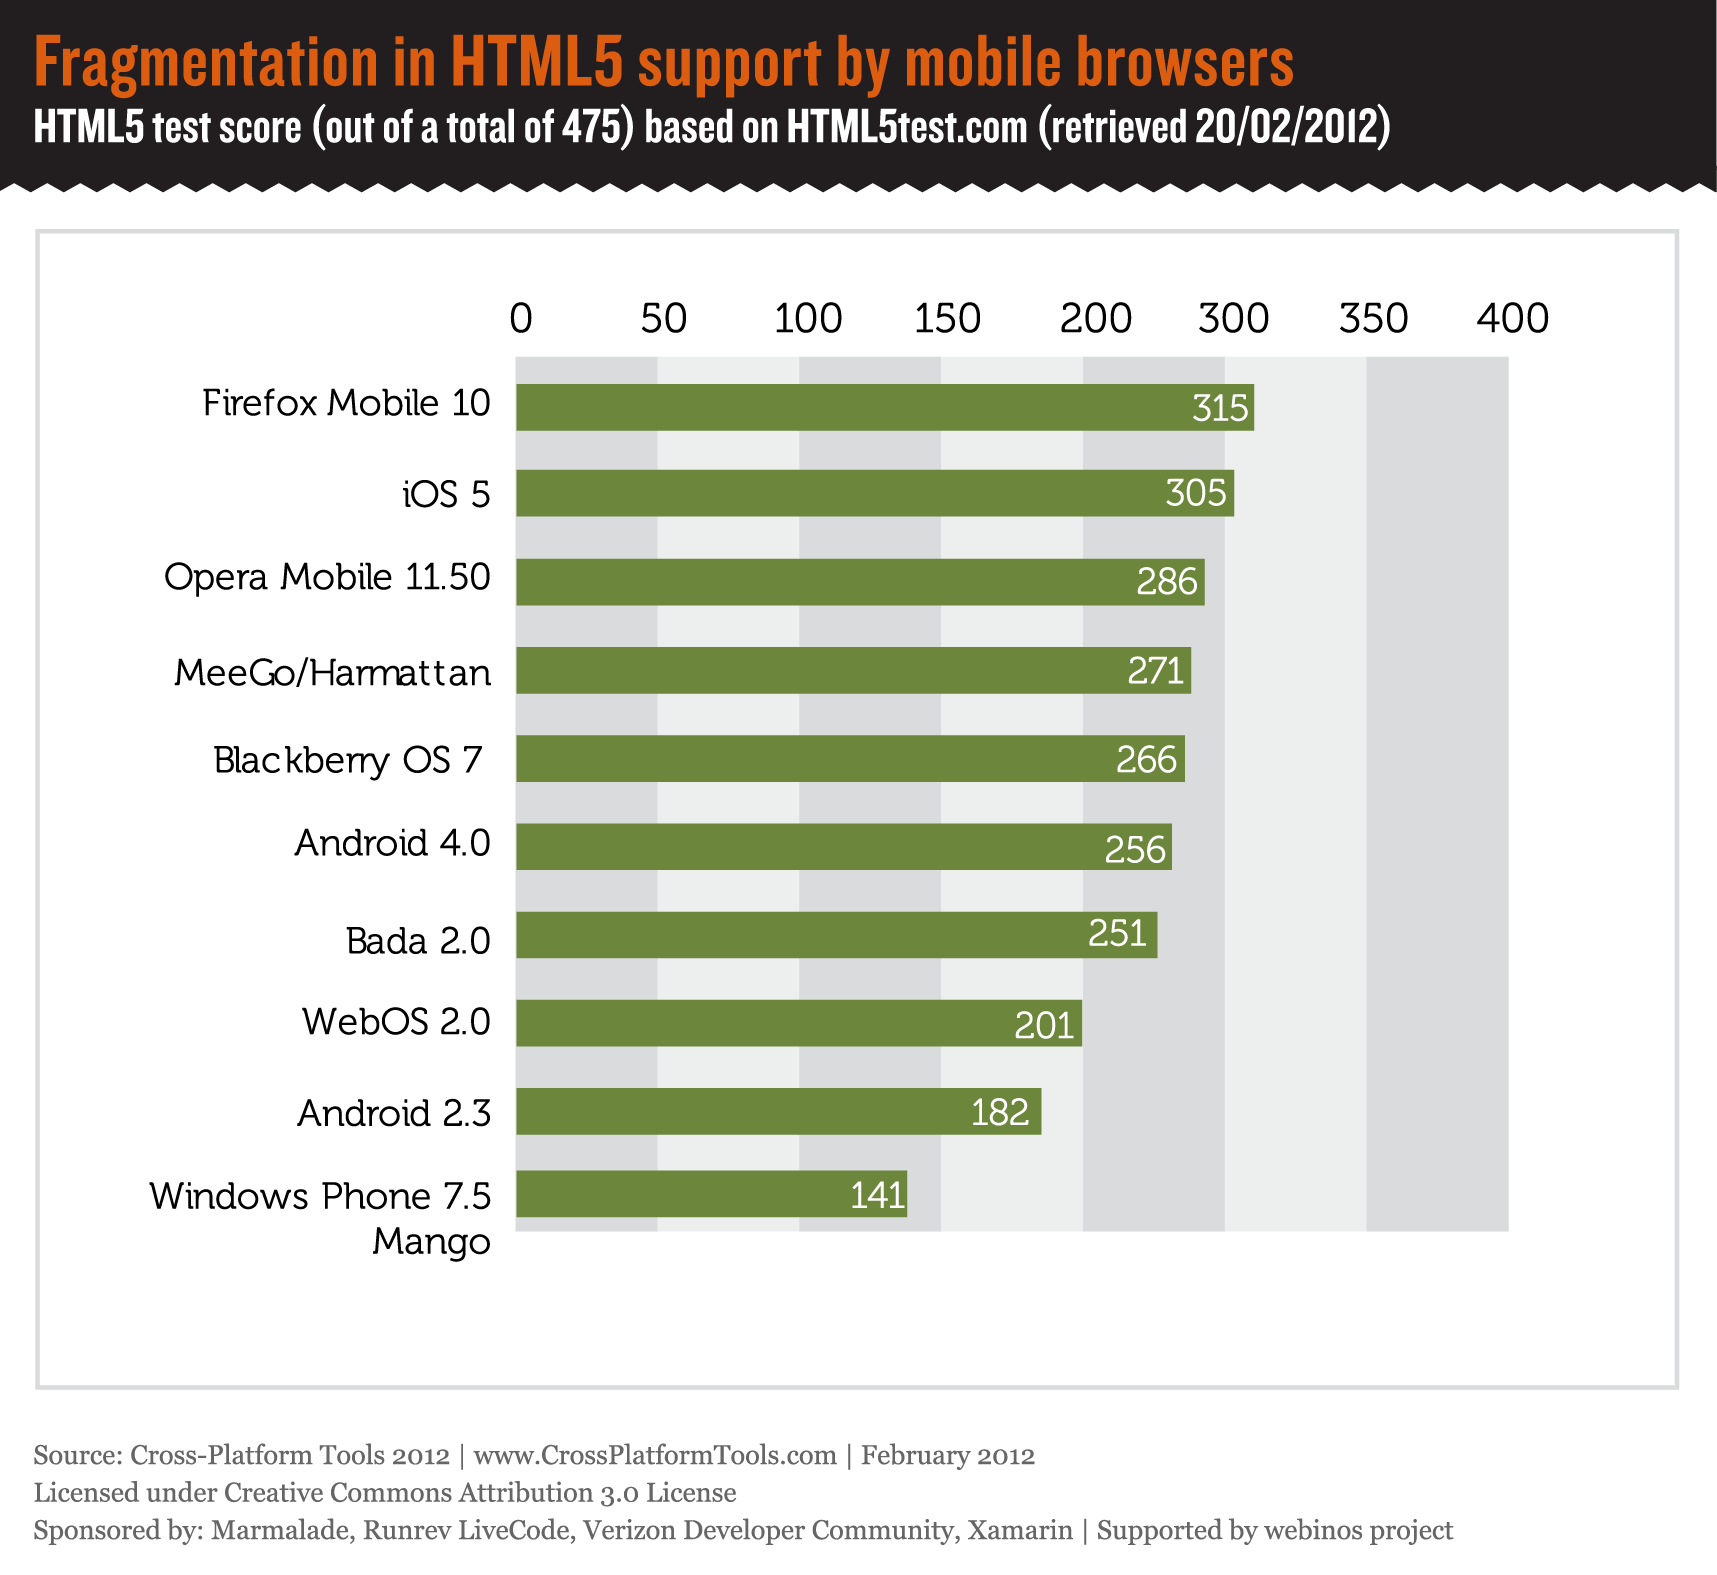
\includegraphics[width=1.0\textwidth]{html5browser.png}
\caption{Podpora HTML5 standardů v mobilních prohlížečích \cite{visionmobile_survey}}
\label{fig:HTML5mobilniprohlizece}
\end{figure}

\subsection{Náročnost vývoje}
I když jsme v benefitech multiplatformního přístupu zmínili, že díky použití webových technologií je samotný vývoj jednodušší, průzkum společnosti VisionMobile \cite{visionmobile_survey} prokázal, že právě strmě stoupající náročnost vývoje je častým důvodem k zavržení multiplatformního nástroje. Zdá se tedy, že s multiplatformními nástroji snadno vyvinete jednodušší aplikaci, ale komplexnější úkoly již představují větší výzvu.

\section{Přístupy k multiplatformnímu vývoji mobilních aplikací}
Dosud jsme hovořili o mutliplatformním vývoji, jako by se jednalo o monolitický celek. V rámci něj však existuje celá řada přístupů, které se od sebe liší technicky i filozoficky. V této části se tedy zaměříme právě na stručný popis těch nejpoužívanějších přístupů, které multiplatformní vývoj nabízí.

\subsection{Javascriptové frameworky}
Do této rodiny řadíme například známý framework jQuery Mobile či Sencha Touch. Jedná se o frameworky, které umožňují webovým vývojářům snadno vyvíjet dotyková rozhraní svých webových aplikací. Například jQuery Mobile poskytuje možnosti jak definovat vzhled stránky a jednotlivé elementy způsobem, který umožní jejich bezproblémové zobrazení na jakémkoliv dotykovém zařízení. Nesnaží se však simulovat nativní vzhled ovládacích prvků na jednotlivých platformách, narozdíl třeba od nástroje Kendo UI.

\paragraph{Zástupci}
\begin{enumerate}
	\item jQuery Mobile
	\item Sencha Touch
	\item Kendo UI
	\item DHTMX Touch
	\item iUI
	\item Cocos2D (hry)
\end{enumerate}

\subsection{Aplikační továrny}
Aplikační továrny jsou velice moderní přístupem, jak tvořit mobilní aplikace. Slovo „tvořit“ je skutečně na místě, neboť při využití těchto nástrojů není třeba žádných znalostí programovacích jazyků (tedy ani HTML, CSS a JavaScriptu). Aplikace jsou tvořeny uživatelem pomocí skládání vizuálních elementů v nějakém (většinou webovém) WYSIWYG editoru. V případě potřeby může uživatel doplnit chybějící logiku pomocí JavaScriptu.

Jedním z nejznámějších zástupců této skupiny je Tiggzi. Tiggzi je poměrně komplexní nástroj, který v sobě kombinuje javascriptový framework jQuery Mobile, webové technologie HTML, CSS a JavaScript a hybridní framework PhoneGap, který umožňuje exportovat aplikace vytvořené v Tiggzi do binárních souborů, které je následně možno publikovat na oficiálních tržištích v rámci jednotlivých platforem.

Tiggzi nabízí uživatelům webový nástroj App builder, kde je možno si velmi jednoduše („drag \& drop“[k]) poskládat uživatelské rozhraní aplikace z předdefinovaných UI komponent. Pokud by vám předdefinovné funkce nestačily, můžete si chybějící funkcionalitu dopsat pomocí JavaScriptu. Díky využití hybridního frameworku PhoneGap může uživatel ve své aplikaci přistupovat k nativním funkcím telefonu. Pro tvůrce aplikací jsou připraveny také nástroje pro snadné připojování k REST API služeb třetích stran. Vaše aplikace tak může snadno získávat data například z Twitteru. Tiggzi dále nabízí nástroje pro testování aplikací, databázové úložiště a další. Je však třeba zmínit, že za použití Tiggzi je třeba zaplatit.

\paragraph{Další zástupci}
\begin{enumerate}
	\item AppMkr
	\item Wix mobile
	\item Spot Specific
	\item Games Salad
\end{enumerate}

\subsection{Hybridní frameworky}
Tento druh multiplatformních nástrojů si popíšeme jen velmi stručně, neboť je mu věnována celá následující kapitola XY. Jedná se o řešení, které umožňuje vývojářům vytvářet aplikace čistě pomocí webových jazyků. Hlavní předností těchto frameworků jsou knihovny napsané v nativních jazycích dané platformy, které vývojářům poskytují tzv. most, pomocí kterého mohou přistupovat k nativním funkcím telefonu jako jsou notifikace, fotoaparát, akcelerometr a podobně. Tyto funkce jsou jim přístupné pomocí JavaScriptového API.
% TODO dodělat reference na kapitoly
Nejznámějším příkladem tohoto přístupu je hybridní framework PhoneGap, kterému se budeme podrobně věnovat v kapitole XY.

\paragraph{Další zástupci}
\begin{enumerate}
	\item Trigger.io
	\item Sencha Touch (v2)
	\item MoSync
\end{enumerate}

\subsection{Runtime}
Tvůrci runtime frameworků se snaží k věci přistupovat trochu jinak. Pokud využíváte takový nástroj, tak vlastně píšete nativní aplikaci, avšak místo nativního jazyka používáte JavaScript. Aplikace se spouští jako nativní, nepotřebuje k tomu prostředníka v podobě webového prohlížeče. Jednou ze zásadních výhod tohoto přístupu je, že při vývoji používáte nativní UI elementy. Není nutné tedy nic napodobovat jako v případě hybridních frameworků a výkon takto napsaných aplikací tak bývá v konečném důsledku rychlejší.

\begin{figure}\centering
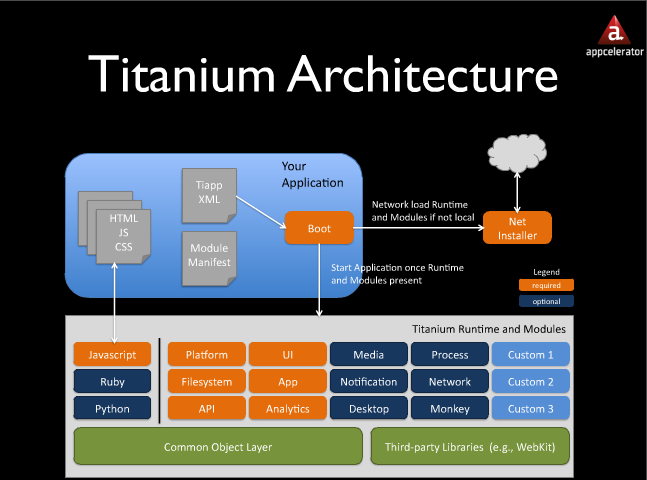
\includegraphics[width=1.0\textwidth]{titanium_architecture.png}
\caption{Architektura runtime frameworku Titanium \cite{architecture_titanium}}
\label{fig:TitaniumArchitecture}
\end{figure}

Pro správné pochopení tohoto principu si můžeme popsat, jak funguje nejznámější zástupce tohoto přístupu – nástroj Appcelerator Titanium. Uživatel v něm píše aplikaci čistě pomocí JavaScriptu, kterýžto zdrojový kód je následně zabalen do nativních binárních souborů určených pro každou z platforem. Při spuštění je použit JavaScriptový interpreter (v iOS JavaScriptCore, v Androidu a Blackberry Mozilla Rhino), který interpretuje váš kód za běhu. Pro volání nativních komponent a hardwarových funkcí telefonu je použito Titanium API, které je napsáno pomocí nativních jazyků a uživatel k němu přistupuje přes volání JavaScriptových funkcí. Appcelerator tvrdí, že 80 \% kódu je možno použít při vývoji mutace aplikace pro jinou platformu \cite{building_apps_titanium}. Hlavním rozdílem oproti hybridním frameworkům je tedy běh aplikací bez nutnosti spouštět webový prohlížeč. O pravé nativní aplikace se však ani v tomto případě nejedná, ač se tím někteří (např. Appcelerator) rádi chlubí. V tomto případě jde spíše o marketingový termín.

Pojďme se seznámit s nástrojem Appcelerator trochu blíže. Krom open-source SDK, které poskytuje více než 5000 API volání pro přístup k nativním prvkům mobilních platforem, je součástí celého řešení i IDE na bázi nástroje Eclipse a MVC framework pro snazší vývoj. Dále je možno využít cloudových služeb pro údržbu a testování aplikací. Pomocí nich lze například posílat push-notifikace, integrovat sociální sítě, posílat e-maily přímo z aplikace apod \cite{appcelerator_features}. Příjemná je i možnost statistického zobrazení dat o používání aplikace uživateli – obdoba Google Analytics. 

Appcelerator se zaměřuje především na webové vývojáře, které se snaží přesvědčit zejména díky lepšímu výkonu oproti aplikacím napsaným pomocí hybridních frameworků jako je PhoneGap \cite{appcelerator_vs_phonegap}. Z výzkumu \cite{visionmobile_survey} vyplývá, že uživatelé si vybírají Appcelerator zejména kvůli nízké ceně, přístupu k hardwarovým funkcím telefonu a širokým možnostem úpravy UI jejich aplikace. Naopak velká část z nich by ocenila ještě lepší optimalizaci orientovanou na jednotlivé platformy.

\paragraph{Další zástupci}
\begin{enumerate}
	\item Adobe Flex/Air
	\item Corona
	\item AppMobi
	\item Unity (Hry)
\end{enumerate}

\subsection{Překladače zdrojových kódů}
Další možností je nechat si přeložit zdrojový kód své aplikace do nativního jazyka dané platformy, případně do nějakého mezikódu či strojového jazyka. Nezřídkakdy jsou překladače zdrojových kódu používány současně s nějakým runtime nástrojem. Tyto nástroje cílí především na zkušené vývojáře, kteří potřebují vyvíjet komplexní aplikace pro více platforem s vysokou úrovní aplikační logiky.

Známým nástrojem z tohoto okruhu je například Marmalade. Marmalade umožňuje vývojářům psát aplikace v jazycích C či C++, který je následně přeložen do nativního jazyka některé z podporovaných platforem. Těch je celá řada, od iOS, Androidu přes Samsung Bada a Blackberry až po dekstopové Windows \cite{marmalade}. Chybí však podpora pro Windows Phone. Pro přístup k nativním funkcím telefonu poskytuje Marmalade SDK API. SDK obsahuje ale i další užitečné nástroje jako je například debugger, UI builder a další.

Podle výzkumu \cite{visionmobile_survey} si vývojáři vybírají Marmalade především proto, že je velmi vhodný na vývoj her. Oceňují na něm také vysoký výkon, který jde pravděpodobně na vrub zejména nízké úrovni abstrakce. Na druhou stranu je u uživatelů poptávka po více možnostech licencování. Používání Marmalade je totiž placeno.

\paragraph{Další zástupci}
\begin{enumerate}
	\item MoSync
	\item Eqela
	\item XMLVM
	\item Bedrock
\end{enumerate}